% 必要な項目ができた場合は適宜サブセクションを追加してください
%\include{begin}

% イベント名を記入する
\section{受付(バスに乗るまで)}


% 日時と場所を記入する
% 時刻は4桁で記入すること!
\subsection{日時・場所}

\begin{tabular}{p{2zw}rp{38zw}}
日時 & : & 2019年4月5日(金) 10:15 $\sim$ 12:10\\
場所 & : & 受付用部屋(K101),東ロータリー (バス乗り場)
\end{tabular}


% 目的を記入する
\subsection{タイムスケジュール}
\begin{longtable}{p{3zw}p{39zw}}
10:15 & \textbf{◎ 受付準備開始} \\
      & \ \  \underline{全スタッフ (先遣隊・後遣隊以外)} \\
      & \ \  \ \ \ \textbullet \ \ 自分の荷物をK101に運ぶ \\
      & \ \  \ \ \ \textbullet \ \ K101の通路に椅子等が置いてある場合は,移動しやすいように片付ける \\
      & \ \  \ \ \ \textbullet \ \ K101にあらかじめ受付と関係のない忘れ物がないか確認しておく \\

      & \ \  \underline{A109物品見張り:別役,生野,斎藤, 新田} \\
      & \ \  \ \ \ \textbullet \ \ 自分の荷物はA109に置いておく\\
      %& \ \  \ \ \ \textbullet \ \ ワゴン車が到着するまで,A109で待機する\\
      %& \ \  \ \ \ \textbullet \ \ ワゴン車(教務の二人)が9:30に到着予定 \\
      & \ \  \ \ \ \textbullet \ \ 西森車が到着次第,別役,斎藤,新田は西森車に荷物を搬入する(生野は部屋に残り見張りを続ける) \\
      & \ \  \ \ \ \textbullet \ \ 搬入後,残っている物品を報告slackで連絡し,必要がない物品を吉田研究室に運ぶ \\
      & \ \  \ \ \ \textbullet \ \ A109に物品が残っていないことを確認し,自分の荷物を持って別役,斎藤,生野,新田はK101に移動する \\

      & \ \  \underline{受付担当:伊崎,青山,吉田,江川} \\
      & \ \  \underline{補助担当:高島,日下,小谷,立岩,渡辺,高橋(慎),石野,東} \\

      & \ \  \ \ \ \textbullet \ \ 学籍番号を示した紙を机の上に貼る\\
      & \ \  \ \ \ \textbullet \ \ 名簿とボールペンを机に並べる\\
      & \ \  \ \ \ \textbullet \ \ 名札を机に並べる\\
      & \ \  \ \ \ \textbullet \ \ 集金ボックスとおつり用のお金を机に置く\\
      & \ \  \ \ \ \textbullet \ \ 準備が終了したら,受付開始まで待機する \\

      & \ \  \underline{統括担当:藤沢,新川} \\
      & \ \  \ \ \ \textbullet \ \ ホワイトボードにバス号車ごとの新入生の配置を書く(図\ref{fig:uketsuke_k101Haichi}参照) \\
      & \ \  \ \ \ \textbullet \ \ ホワイトボードに以下の諸注意を書く \\

      & \ \ 【諸注意】\\
      & \ \  \ \ \ - 学籍番号から各自バスの号車を確認し,受付に移動する(バス号車の区別が書かれた紙をテーブルに貼っておく) \\
      & \ \  \ \ \ - バスの乗り込みは12:00から \\
      & \ \  \ \ \ - バスが来るまで荷物は各自で持っておく \\
      & \ \  \ \ \ - 荷物は各自座席に持って行くこと(ただし,大きい荷物(ボストンバック以上)があればバスのトランクに入れる) \\
      & \ \  \ \ \ - 野外炊事,就寝部屋,イベントのグループ,バスの号車は名札に書いている \\
      & \ \  \ \ \ - トイレにいく場合はスタッフに声をかけ,出口(東側の扉)から出る \\
      & \ \  \ \ \ - 必要のある場合以外は教室から出ない \\
      & \ \  \ \ \ - 教室から出るときに忘れ物がないか確認する \\
      & \ \  \ \ \ - 受付を済ませた新入生は名札を身につけ,しおりの9ページにある自己紹介カードを記入する \\
      & \ \  \ \ \ - 食堂でご飯を食べたい新入生はスタッフに声をかけ,11:55までにK101に戻って来る \\

      & \ \  \underline{司会担当:塩谷, 中島, 丸田, 高橋(龍), 北村, 藤田} \\
      & \ \  \ \ \ \textbullet \ \ バス内企画やスケジュールの最終確認を行う\\

      & \ \  \underline{後遣隊:西森,藤沢} \\
      & \ \  \ \ \ \textbullet \ \ 自分の荷物を後遣隊の車にのせる \\\\
      & \ \  \ \ \ \textbullet \ \ 宴の荷物を後遣隊に乗せる \\\\


11:00 & \textbf{◎ 見回り} \\
      & \ \  \underline{司会:塩谷, 中島, 丸田, 高橋(龍), 北村, 藤田} \\
      & \ \  \underline{救護車:堀川,貞松} \\
      & \ \  \underline{後遣隊:西森,藤沢} \\
      & \ \  \underline{物品見張り:別役,生野,斎藤, 新田} \\
            & \ \  \underline{見回り担当:角原} \\
      & \ \  \ \ \ \textbullet \ \ K棟周辺でK101の位置を知らせる \\\\


11:15 & \textbf{◎ K101への誘導準備} \\
      & \ \  \underline{救護車:堀川,貞松} \\
      & \ \  \underline{後遣隊:西森,藤沢} \\
      & \ \  \ \ \ \textbullet \ \ K101の入口付近,出口付近,教室内で待機しておく \\
      %& \ \  \ \ \ \textbullet \ \ 小野は高橋(錬)と豊山くん(新入生)の顔合わせをする\\\\


11:30 & \textbf{◎ 新入生の受付開始 } \\
      & \ \  \underline{受付担当:伊崎,青山,吉田} \\
      & \ \  \underline{補助担当:高島,日下,小谷,渡辺,石野,東} \\
      & \ \  \ \ \ \textbullet \ \ 新入生が受付にきたら名前を聞いて名簿のチェック欄にチェックをして,参加費(500円)を徴収する \\
      & \ \  \ \ \ \textbullet \ \ 事前アンケートで不備があった人に入浴の確認をする(受付は事前にチェックしておく) \\
      & \ \  \ \ \ \textbullet \ \ 新入生に名札を渡す \\
      & \ \  \ \ \ \textbullet \ \ 新入生の荷物でトランクに入れる必要があった場合,新入生にタグを渡して名前と野外炊事の班を記入してもらいその荷物にタグをつける \\
      & \ \  \ \ \ \textbullet \ \ その後,各列の席に座らせ,ホワイトボードの諸注意を読んでおくように伝える \\
      & \ \  \ \ \ \textbullet \ \ 大きい荷物の判断は受付担当が行う \\

      & \textbf{◎ 先生の受付開始} \\
      & \ \  \underline{受付担当:江川} \\
      & \ \  \underline{補助担当:立岩,高橋(慎也)} \\
      & \ \  \ \ \ \textbullet \ \ 先生は予定時間より早めに来られる可能性があるため注意する \\
      & \ \  \ \ \ \textbullet \ \ 名簿のチェック欄にチェックをしてから名札を渡す \\
      & \ \  \ \ \ \textbullet \ \ 参加費 (2000円)を徴収する \\
      & \ \  \ \ \ \textbullet \ \ 先生の荷物を受け取り,野外炊事の班を記入したタグを付けてK101に置いておく(荷物を見張る) \\
      & \ \  \ \ \ \textbullet \ \ 受付が終了した先生はK101で待機してもらう \\

      & \textbf{◎ K101への誘導・アナウンス開始} \\
      & \ \  \underline{統括担当:藤沢,新川} \\
      & \ \  \ \ \ \textbullet \ \ K101の先生方と待機している新入生に対して,適宜,諸注意をアナウンスする \\
      & \ \  \ \ \ \textbullet \ \ トイレには行っておくよう連絡する \\
      & \ \  \ \ \ \textbullet \ \ 受付を済ませた後に食堂に行きたい新入生がいたら,メモを取っていってもらう \\
      & \ \  \ \ \ - このとき11:55までにK101に戻って来るように伝える \\
      
      & \ \  \underline{救護車:堀川,貞松} \\
      & \ \  \underline{後遣隊:西森,藤沢} \\
      & \ \  \ \ \ \textbullet \ \ K101の入口のドアを開ける \\
      & \ \  \ \ \ \textbullet \ \ K101の出口側の通路付近で入口が東側(食堂側)であることを促す \\
      & \ \  \ \ \ \textbullet \ \ K101に入ってきた新入生に対し,各受付がバスの号車ごとに分かれていることを説明しながら誘導する \\
      & \ \  \ \ \ \textbullet \ \ 新入生がトイレにいく場合は出口(西側)から行かせる \\

      & \textbf{◎ バス司会者見回り終了} \\
      & \ \  \underline{司会担当:塩谷, 中島, 丸田, 高橋, 北村, 藤田} \\
      & \ \  \ \ \ \textbullet \ \ 自分の荷物を持ち,東ロータリーへ移動し,バスが来るのを待つ \\\\

11:40 & \textbf{◎ バス到着} \\
      & \ \  \underline{司会担当:塩谷, 中島, 丸田, 高橋, 北村, 藤田} \\
      & \ \  \ \ \ \textbullet \ \ バス(運転手:???, ???, ???が到着するのでバス司会は待機しておく \\
      & \ \  \ \ \ \textbullet \ \ 担当バスの運転手に挨拶をする \\
      & \ \  【確認事項】\\
      & \ \  \ \ \ - バス内での飲食の確認 \\
      & \ \  \ \ \ - バス内でのマイクの使用 \\
      & \ \  \ \ \ - その他乗車上の注意 \\
      & \ \  \ \ \ - 自分の荷物をバスのトランクにのせる \\
      & \ \  \ \ \ - 司会担当は,運転手との挨拶後,新入生が来るまでにマイクなどを確認する \\
      & \ \  \ \ \ - 司会担当は,バスの運転手と休憩場所の確認と到着時間の確認をし,確認内容を報告slackに連絡する \\

      & \ \  \underline{司会担当1:藤田,中島,丸田} \\
      & \ \  \ \ \ \textbullet \ \ 集合場所に移動し,バスが来たことを補助担当に伝える \\

      & \ \  \underline{司会担当2:北村,高橋,塩谷} \\
      & \ \  \ \ \ \textbullet \ \ バスのドア付近で待機し,乗車確認の準備をする \\\\


12:00 & \textbf{◎ 新入生の受付終了} \\
      & \ \  \underline{司会担当1:藤田,中島,丸田} \\
      & \ \  \underline{補助担当:高島,日下, 小谷, 渡辺,石野,東} \\
      & \ \  \ \ \ \textbullet \ \ バス到着の連絡がきたら,補助担当は自分の荷物を持ち,司会担当と一緒に新入生をバスへ誘導する \\
      & \ \  \ \ \ \textbullet \ \ 混雑を防ぐため,3号車,2号車,1号車の順で誘導する \\
      & \ \  \ \ \ \textbullet \ \ 新入生が大きい荷物を持ってきた場合は,バスのトランクに荷物をのせる \\
      & \ \  \ \ \ \textbullet \ \ 補助担当は自分の荷物をバスのトランクにのせる \\
      & \ \  \ \ \ \textbullet \ \ 誘導後,司会担当はそのままバスへ,補助担当は,K101に戻る \\

      & \ \  \underline{司会担当2:北村,高橋(龍),塩谷} \\
      & \ \  \ \ \ \textbullet \ \ バスの入口付近で乗車確認リストを用いて,乗車する新入生のチェックを行う \\
      & \ \  \ \ \ \textbullet \ \ 奥からつめて座るように伝える \\
      & \ \  \ \ \ \textbullet \ \ 新入生の女子が1人で来たときは,一旦待機させ,他の女子と隣になるように乗せる \\
      & \ \  \ \ \ \textbullet \ \ バス酔いや体調不良がある人は前方に座らせる \\
      & \ \  \ \ \ \textbullet \ \ 全員が乗車したら,各バスの乗車人数を確認する \\

      & \ \  \underline{受付担当:伊崎,吉田,青山} \\
      & \ \  \ \ \ \textbullet \ \ 12:00以降に来た新入生は,受付をした後,集合場所で待機させておく\\
      & \ \  \ \ \ \textbullet \ \ 各号車ごとに受付を済ませた新入生の人数をまとめる \\

      & \ \  \underline{救護車:堀川,貞松} \\
      & \ \  \ \ \ \textbullet \ \ 自分の荷物を持ち,車を東ロータリーに移動させる\\
      & \ \  \ \ \ \textbullet \ \ 出発の準備をする\\

      & \textbf{◎ 先生の受付終了} \\
      & \ \  \underline{受付担当:江川} \\
      & \ \  \underline{補助担当:立岩,高橋(慎)} \\
      & \ \  \ \ \ \textbullet \ \ 自分の荷物を持つ \\
      & \ \  \ \ \ \textbullet \ \ 新入生の誘導が完了次第,先生をバスに誘導する \\
      & \ \  \ \ \ \textbullet \ \ 全て報告slackを用いて状況を把握し,適宜動く \\\\

12:05 & \textbf{◎ 新入生の乗車確認} \\
      & \ \  \underline{受付担当:伊崎,吉田,青山} \\
      & \ \  \ \ \ \textbullet \ \ 各号車ごとに受付を済ませた新入生の人数をまとめる \\

      & \ \  \underline{司会担当:塩谷, 中島, 丸田, 高橋, 北村, 藤田} \\
      & \ \  \ \ \ \textbullet \ \ 各バスの司会者は,各バスの受付担当と電話で連絡を取り,乗車人数と合うかを確認する \\

      & \ \  【乗車人数があわないとき】\\
      & \ \  \ \ \ \textbullet \ \ 受付の名簿にチェックがあるが,バスの乗車確認リストにチェックがない場合 \\
      & \ \  \ \ \ \ \ \ \ \ →補助担当が大学内を探す \\
      & \ \  \ \ \ \textbullet \ \ バスの乗車確認リストにチェックがあるが,受付の名簿にチェックがない場合 \\
      & \ \  \ \ \ \ \ \ \ \ →司会担当がバス内にアナウンスし,その新入生が乗車しているか再確認する \\

& \ \  \underline{補助担当:石野,高島,渡辺,日下,東,小谷,立岩,高橋(慎)} \\
& \ \  \underline{見回り担当:角原,渡辺,別役,斎藤,生野,新田} \\
      & \ \  \ \ \ \textbullet \ \ 先生方の荷物を各バスに運ぶ \\
      & \ \  \ \ \ \textbullet \ \ 運んだ後はそのままバスで待機する \\
      & \ \  \ \ \ \textbullet \ \ 荷物が積み終わったら, 吉田が報告slackに連絡する \\

& \ \  \underline{受付補助担当:貞松} \\
      & \ \  \ \ \ \textbullet \ \ 貞松は先生受付担当の江川から仕事を引き継ぐ \\
      & \ \  \ \ \ \textbullet \ \ 来られた先生の人数をまとめる \\
      & \ \  \ \ \ \textbullet \ \ 先生の受付まわりに忘れ物がないか確認する \\

      & \ \  \underline{司会担当:塩谷, 中島, 丸田, 高橋(龍), 北村, 藤田} \\
      & \ \  \ \ \ \textbullet \ \ バスの入口付近で乗車確認リストを用いて,乗車する先生のチェックを行う \\
      & \ \  \ \ \ \textbullet \ \ 受付担当と連絡を取り,先生の乗車人数があうか確認する \\\\

      & \ \  \underline{後遣隊:西森,藤沢} \\
      & \ \  \ \ \ \textbullet \ \ 藤沢は参加費の計算をする \\
      & \ \  \ \ \ \textbullet \ \ 受付まわりに忘れ物がないか確認する忘れ物がある場合は司会担当と連絡をとり,忘れ物の特徴などをバス内に伝えてもらう早急に対応できそうであれば,忘れ物をバスまで持って行ってもよい \\

      & \textbf{◎ 受付完全終了} \\
      & \ \  \underline{受付担当:伊崎,吉田,青山,江川} \\
      & \ \  \ \ \ \textbullet \ \ 全体の受付を終了する \\
      & \ \  \ \ \ \textbullet \ \ 自分の荷物を持ち,遅刻者を連れてバスへ移動する \\
      & \ \  \ \ \ \textbullet \ \ 自分の荷物をバスのトランクにのせ,バスで待機する \\

      & \ \  \underline{見回り担当:斎藤,角原,渡辺,別役,新田} \\
      & \ \  \ \ \ \textbullet \ \ 自分の荷物を持ち,バスへ移動する \\
      & \ \  \ \ \ \textbullet \ \ 自分の荷物をバスのトランクにのせ,バスで待機する \\

      & \ \  \underline{後遣隊:西森,藤沢} \\
      & \ \  \ \ \ \textbullet \ \ この時間以降の受付は後遣隊が行う \\
      & \ \  \ \ \ \textbullet \ \ 藤沢は参加費を回収する \\
      & \ \  \ \ \ \textbullet \ \ その後,藤沢が物品と参加費を吉田研究室に運ぶ \\\\

12:10 & \textbf{◎ バス・救護車出発} \\
      & \ \  \underline{各スタッフ} \\
      & \ \  \ \ \ \textbullet \ \ バスで移動するスタッフはこの時間までにバスに乗車する \\

      & \ \  \underline{救護車:堀川,貞松} \\
      & \ \  \ \ \ \textbullet \ \ 救護車はバスの後ろを追いかける \\

\end{longtable}

\subsection{人員配置}

\begin{itemize}
\item 受付統括:藤沢,新川
\item A109物品見張り,ワゴン車荷物搬入:別役,生野,斎藤,新田
\item 1号車受付:伊崎
\item 1号車受付補助:高島,石野
\item 2号車受付:吉田
\item 2号車受付補助:日下,渡辺
\item 3号車受付:青山
\item 3号車受付補助:小谷,東
\item 先生受付:江川
\item 先生受付補助:立岩,高橋(慎)
\item 1号車司会:北村,藤田
\item 2号車司会:中島,高橋(龍)
\item 3号車司会:丸田,塩谷
\item 見回り:角原,渡辺
\item 会計:藤沢
\item 救護車:堀川,貞松
\item 後遣隊1:西森,藤沢
\end{itemize}

\subsection{バス号車の配置(最終人数により調整)}
\begin{itemize}
\item  1号車:伊崎,斎藤,生野,高島,高橋(慎),石野
\item  2号車:吉田,立岩,日下,渡辺,別役,新田
\item  3号車:青山,新川,角原,小谷,東,江川
\end{itemize}

%\clearpage

%\begin{figure}[H]
 % \begin{center}
 %   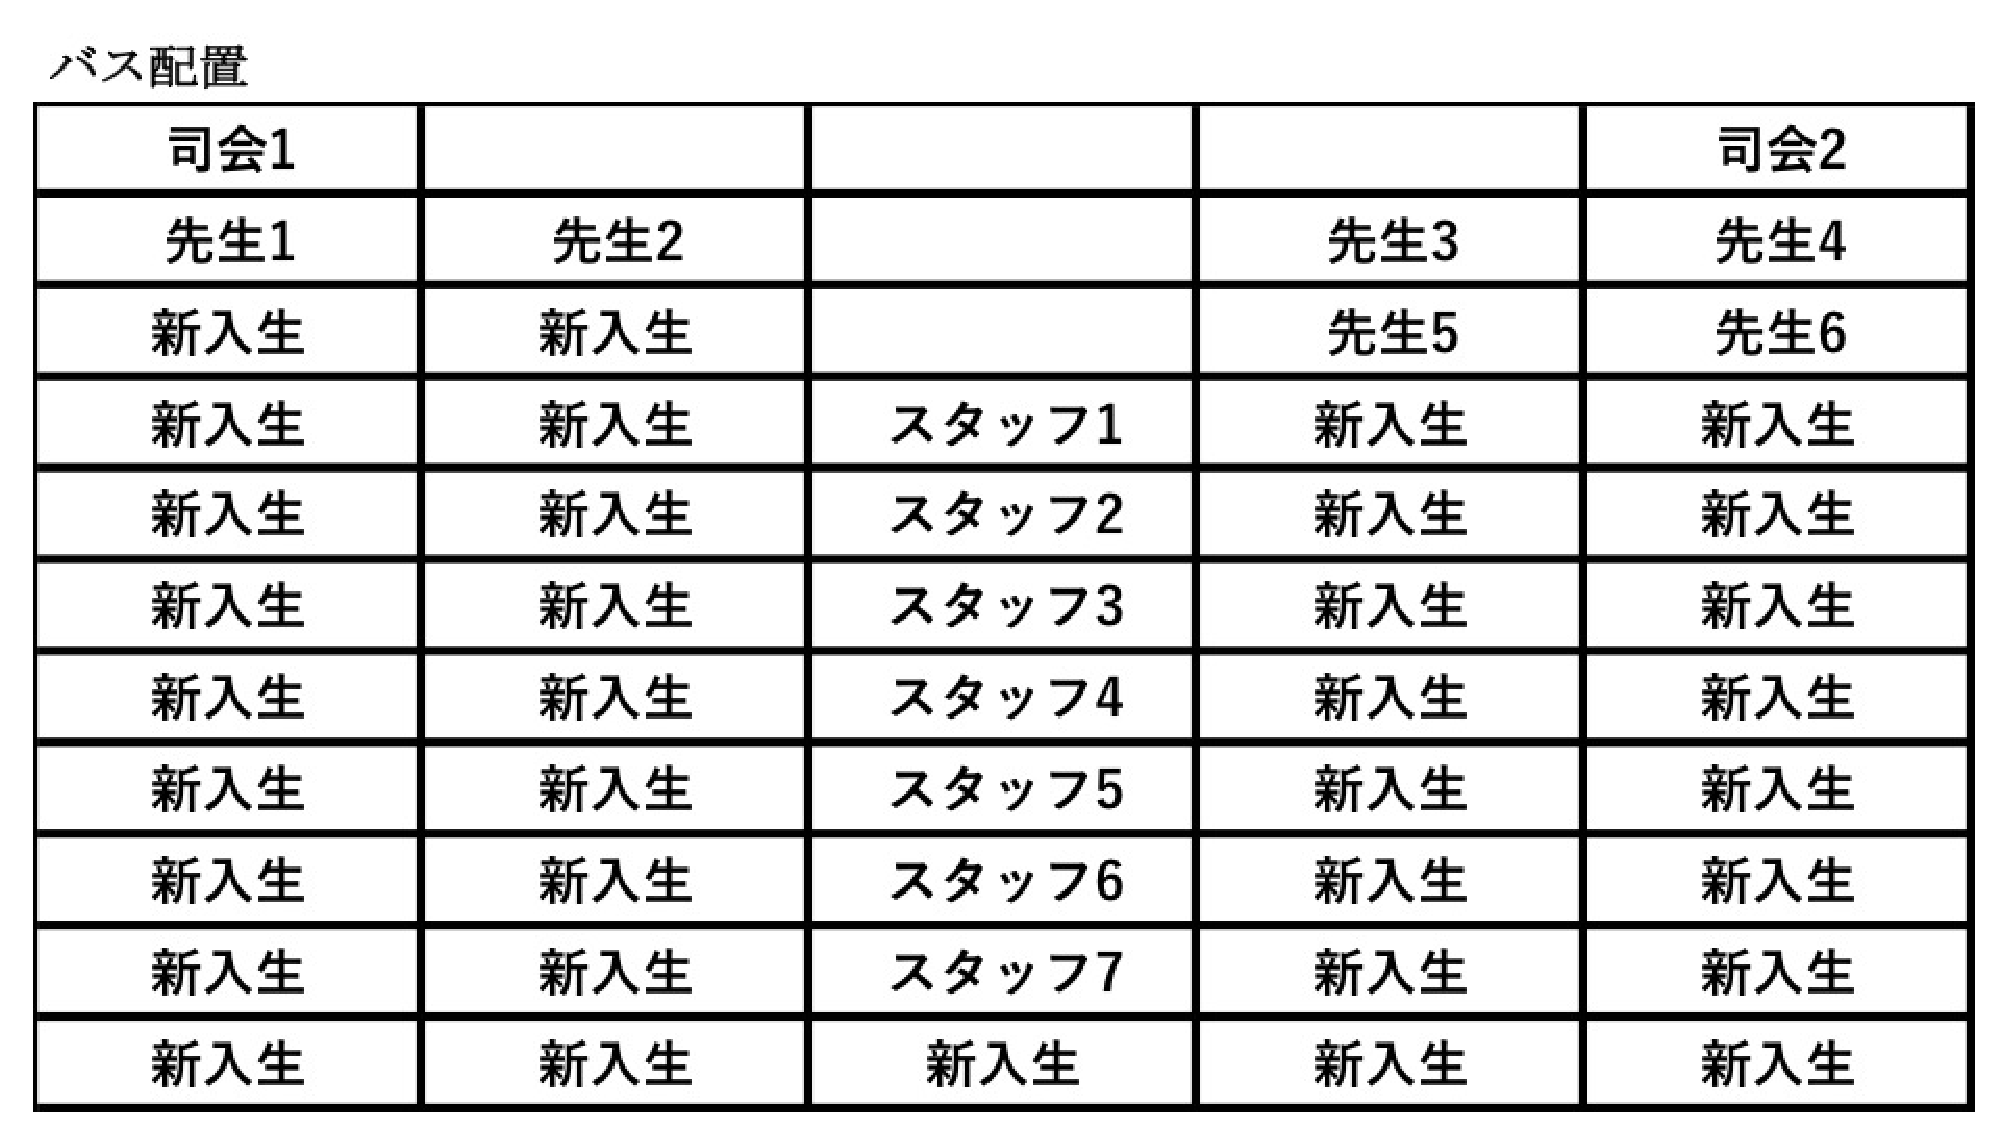
\includegraphics[keepaspectratio, width=15cm]{./04/bus_memberHaichi1.eps}
 %   \caption{バス配置}
 %   \label{fig:bus_memberHaichi1}
%  \end{center}
%\end{figure}

\begin{table}[htb]
  \begin{center}
  \begin{tabular}{|c|c||c||c|c|} \hline
  司会1  & 司会2  &           &        & 先生1 \\ \hline 
  先生2  & 先生3  &           & 先生4  & 先生5 \\ \hline
  新入生 & 新入生 &           & 先生6  & 先生7  \\ \hline
  新入生 & 新入生 & スタッフ1 & 新入生 & 新入生 \\ \hline
  新入生 & 新入生 & スタッフ2 & 新入生 & 新入生 \\ \hline
  新入生 & 新入生 & スタッフ3 & 新入生 & 新入生 \\ \hline
  新入生 & 新入生 & スタッフ4 & 新入生 & 新入生 \\ \hline
  新入生 & 新入生 & スタッフ5 & 新入生 & 新入生 \\ \hline
  新入生 & 新入生 & スタッフ6 & 新入生 & 新入生 \\ \hline
  新入生 & 新入生 & スタッフ7 & 新入生 & 新入生 \\ \hline
  新入生 & 新入生 &  新入生  & 新入生 & 新入生  \\ \hline

  \end{tabular}
\caption{バス内配置}
  \end{center}
\end{table}

\begin{figure}[H]
  \begin{center}
    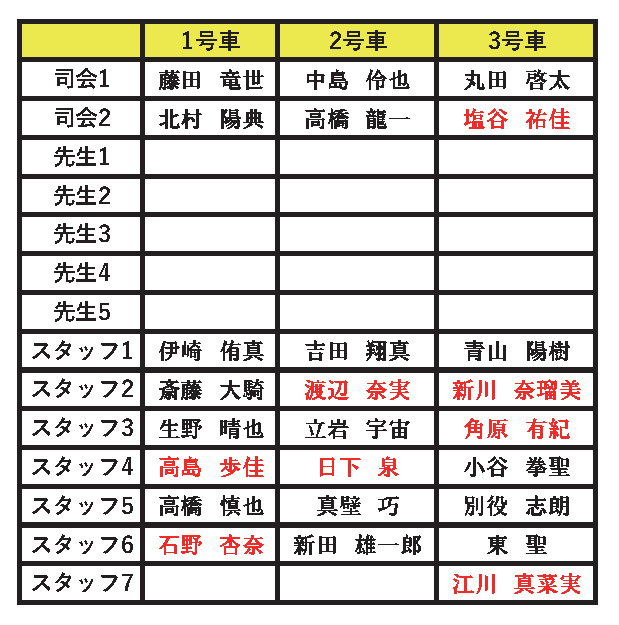
\includegraphics[keepaspectratio, scale=0.9]{./04/bus_memberHaichi2.eps}
    \caption{バス配置}
    \label{fig:bus_memberHaichi2}
  \end{center}
\end{figure}

\subsection{全体配置}
\begin{figure}[H]
  \begin{center}
    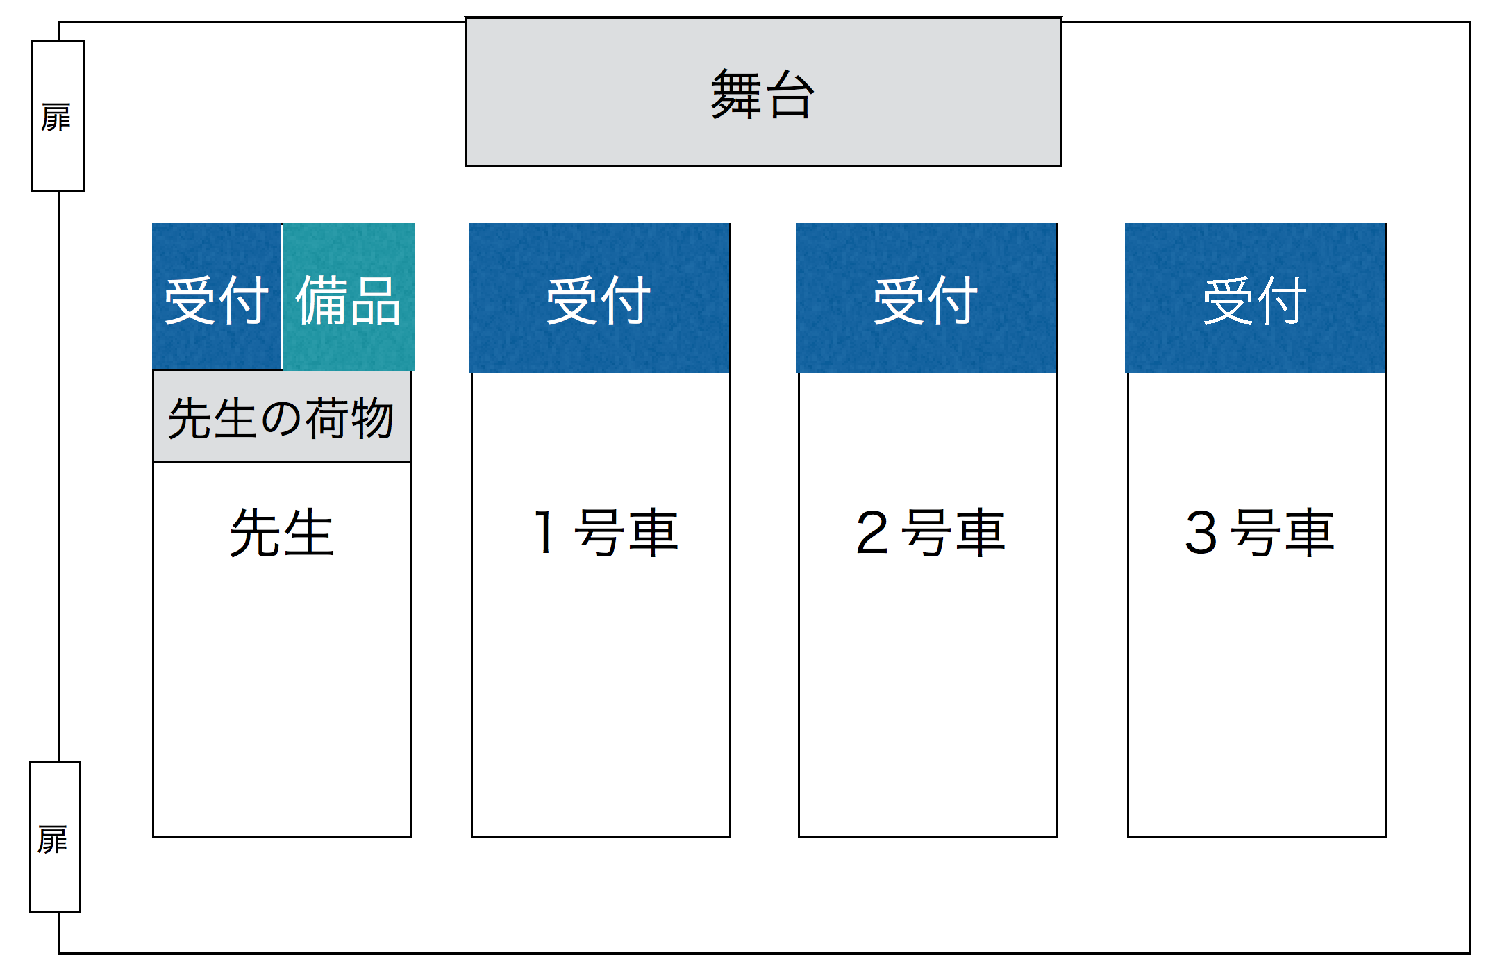
\includegraphics[keepaspectratio, width=10cm]{./04/uketsuke_k101Haichi.eps}
    \caption{K101の全体配置}
    \label{fig:uketsuke_k101Haichi}
  \end{center}
\end{figure}


% イベントに必要な物品と個数を記入する

% 記入例 ・マジックペン 10本


\subsection{必要物品}
\begin{itemize}
\item 名札:人数分
\item 名簿:4部(チェック欄,学籍番号,名前,ふりがなを記載)
\item 名札ケース:人数分
\item しおり:人数分
\item 集金ボックス:4箱
\item おつり用のお金:40枚
\item ボールペン:4本(受付チェック用)
\item ホッチキス:5個(荷物のタグ付け用)
\item 紙:4枚(学籍番号を示した紙3枚,先生用1枚)
\item マスキングテープ:1個(紙を貼るとき用)
\item 荷物用のタグ:人数分(先生・荷物を預けた新入生・スタッフ用)
\item 乗車確認リスト:3部(バスの乗車確認用)
\item 予備のしおり:10部
\end{itemize}


\subsection{備考}
\begin{itemize}
\item K101は10:00から使用できる
\item K101:258席,座席は前から詰めて座るようにする
\item バスのトランクには原則新入生の荷物はのせない ただし,キャリーバッグなど大きい荷物はのせてもよい
\item スタッフの荷物はバスのトランクにのせる ただし,先遣隊・救護車・後遣隊は各自で持っていく 当日集まったとき,スタッフは自分の荷物にタグをつける
\item 会計担当は当日までにおつり用のお金を用意しておく
\item 受付担当はホッチキスとボールペンを用意しておく
\item 受付は速やかに行動する
\item 新入生と関わる一番はじめの場なので明るく元気な挨拶を心がける
\item 新入生のオリエンテーション時に荷物を置ける余裕がないことを知らせておく
\item 人員配置されていないスタッフは,基本的に見回りにまわる
\end{itemize}



% \subsection{連絡事項}
% \begin{table}[h]
% \begin{tabular}{|c|c|c|c|c|} \hline
% 報告者                 & 対象   & 内容                           & タイミング             & 備考   \\ \hline
% 川添                   & 全体   & バスが到着したこと             & バス到着時             &        \\ \hline
% 各バス司会             & 各受付 & 各号車の新入生の乗車人数確認   & 新入生乗車後           & 電話で \\ \hline
% 各バス司会             & 全体   & 新入生の乗車人数を確認したこと & 新入生の乗車人数確認後 &        \\ \hline
% 河野,下出,植田       & 全体   & 新入生の遅刻者の有無           & 新入生の乗車人数確認後 &        \\ \hline
% 各バス司会             & 各受付 & 各号車の先生の乗車人数確認     & 先生乗車後             & 電話で \\ \hline
% 各バス司会             & 全体   & 先生の乗車人数を確認したこと   & 先生の乗車人数確認後   &        \\ \hline
% 領内                   & 全体   & 先生の遅刻者の有無             & 先生の乗車人数確認後   &        \\ \hline
% 司会補助               & 全体   & 先生の荷物の積み込み完了       & 荷物も積み込み完了後   &        \\ \hline
% 手塚,川添,本田,鈴木(夏) & 全体 & 各バス,救護車が出発したこと & バス,救護車出発時     &        \\ \hline
% \end{tabular}
% \end{table}

%\include{end}
